\chapter{Analisi dei Risultati} 

I dati relativi agli indici di prestazione di interesse (tempi di risposta e throughput) misurati 
nelle precedenti fasi di test sono stati in seguito aggregati e visualizzati in forma di grafici. 
Infatti, in base al tipo di test effettuato, tali grafici si suddividono in due categorie: i grafici di 
throughput e tempi di risposta del sistema in stato di instabilit\`a (front server sovraccarico) e 
quelli relativi al sistema in condizione di stazionariet\`a (front server non sovraccarico), ovvero quelli gestiti
attraverso il meccanismo di overload management.

\section{Sistema senza Overload Management}

\subsection{Response Time}

In questo scenario l'utilizzazione del front-end server \'e praticamente uguale a 1, perci\`o 
non riesce a completare tutte le richieste entranti, con la inevitabile 
situazione di veder aumentare indefinitamente la lunghezza della sua coda. Di 
conseguenza il tempo di risposta del sistema tende a divergere all'aumentare del tempo di 
simulazione. Il grafico illustrato di seguito mostra tale scenario:

\begin{figure}[H]
 \centering
 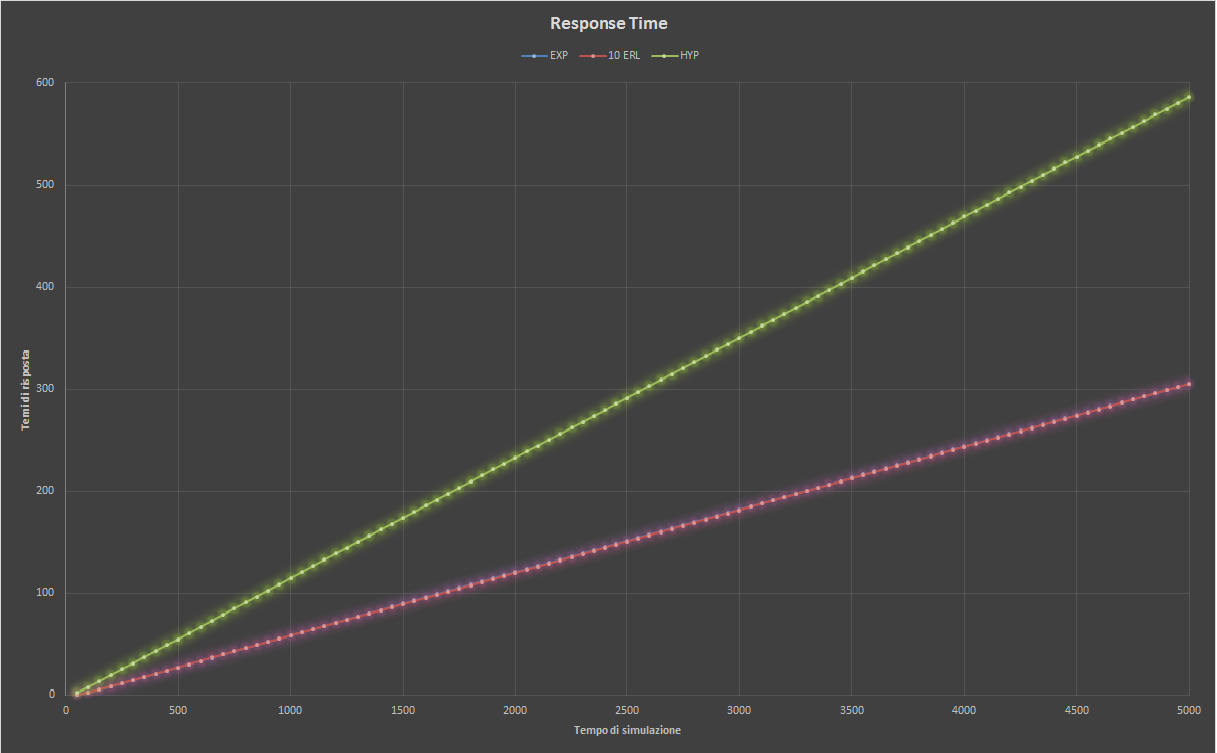
\includegraphics[scale=0.45]{img/responseTime.png}
 \caption[Tempi di risposta del sistema instabile]{Tempi di risposta del sistema instabile}
 \label{fig:Tempi di risposta del sistema instabile}
\end{figure}

Come si intuisce dal grafico sopra riportato, i tempi di risposta si contraddistinguono in base
al tipo di distribuzione dei tempi di servizio del front-end server (iperesponenziale, 10-erlang 
ed esponenziale), e in base all'andamento delle curve dei tempi di risposta, risulta evidente 
come la distribuzione iperesponenziale dei tempi di servizio del front-end risulta peggiore 
che nel caso esponenziale e 10-erlang, dove i tempi rimangono uguali.

Questa sostanziale differenza \`e dovuta al fatto che, nel caso iperesponenziale, avendo 
preimpostato la probabilità \textbf{p=0.1}, la varianza dei tempi di servizio delle richieste risulta 
essere molto elevato con la conseguenza di rallentare notevolmente il front-end server.
Di conseguenza la curva dei tempi di risposta della iper-esponenziale diverge pi\`u 
rapidamente rispetto alle controparti 10-erlang ed esponenziale. Tuttavia il grafico mostra 
anche un aspetto insolito: la curva del tempo di risposta della 10-erlang coincide 
praticamente con la curva dell'esponenziale anche avendo impostato un parametro K=10, 
mentre ci si aspettava, al contrario, un miglioramento dei tempi di risposta rispetto alla curva 
della esponenziale. Probabilmente la scelta del parametro K pari a 10 \'e insufficiente a 
garantire un miglioramento significativo.

\subsection{Autocorrelazione}

L'evidente divergenza dei tempi di risposta del sistema \'e evidenziata anche dalla forte 
correlazione presente dai tempi di risposta delle singole richieste presenti nel sistema. Il 
grafico seguente illustra tale correlazione sulle tre distribuzioni:

\begin{figure}[H]
 \centering
 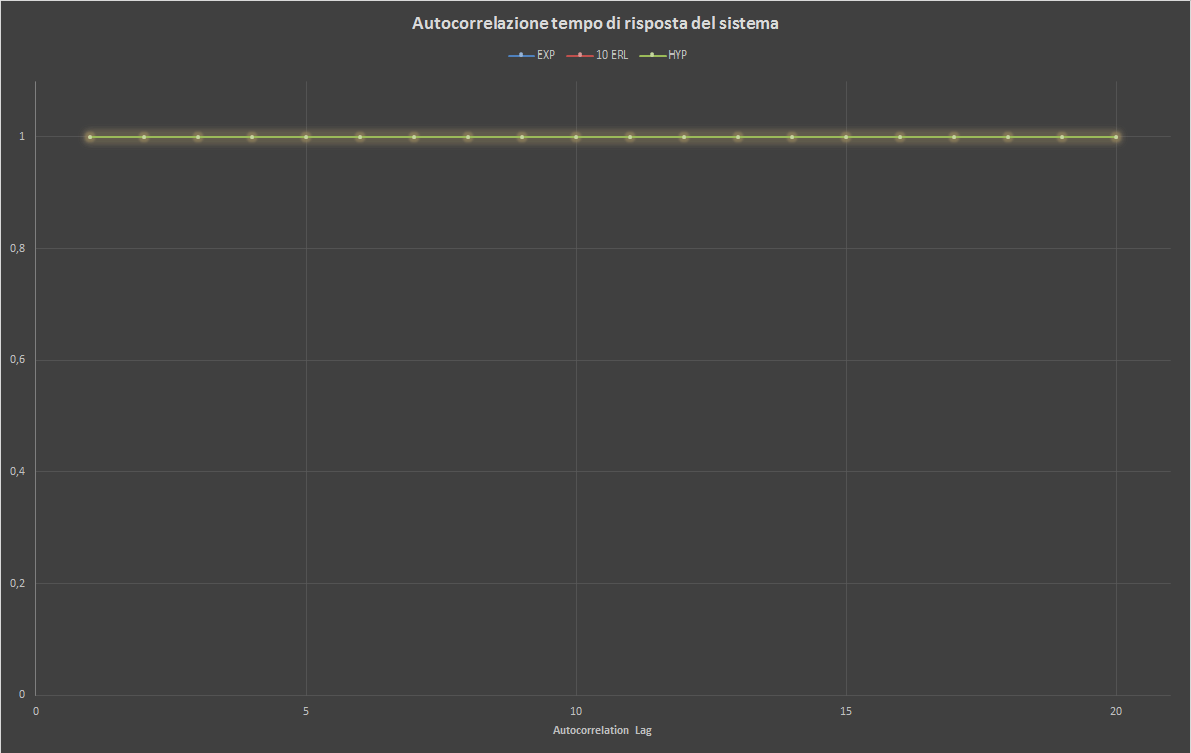
\includegraphics[scale=0.45]{img/autocorrelation.png}
 \caption[Autocorrelazione dei tempi di risposta]{Autocorrelazione dei tempi di risposta}
 \label{fig:Autocorrelazione dei tempi di risposta}
\end{figure}

Dal grafico non si evince bene ma i valori dell'autocorrelazione relativi alla distribuzione
iperesponenziale sono leggermente inferiori rispetto agli altri due casi (nell'ordine di $10^{-2}$)
ma si assestano tutti nell'intorno di 0.9.

\subsection{Useful Throughtput}

Il grafico successivo mostra l'andamento dello useful throughput i cui valori sono stati
misurati dagli stessi test usati per il tempo di risposta del sistema. Anche in questo caso si 
distinguono le diverse distribuzioni dei tempi di servizio del front-end server:

\begin{figure}[H]
 \centering
 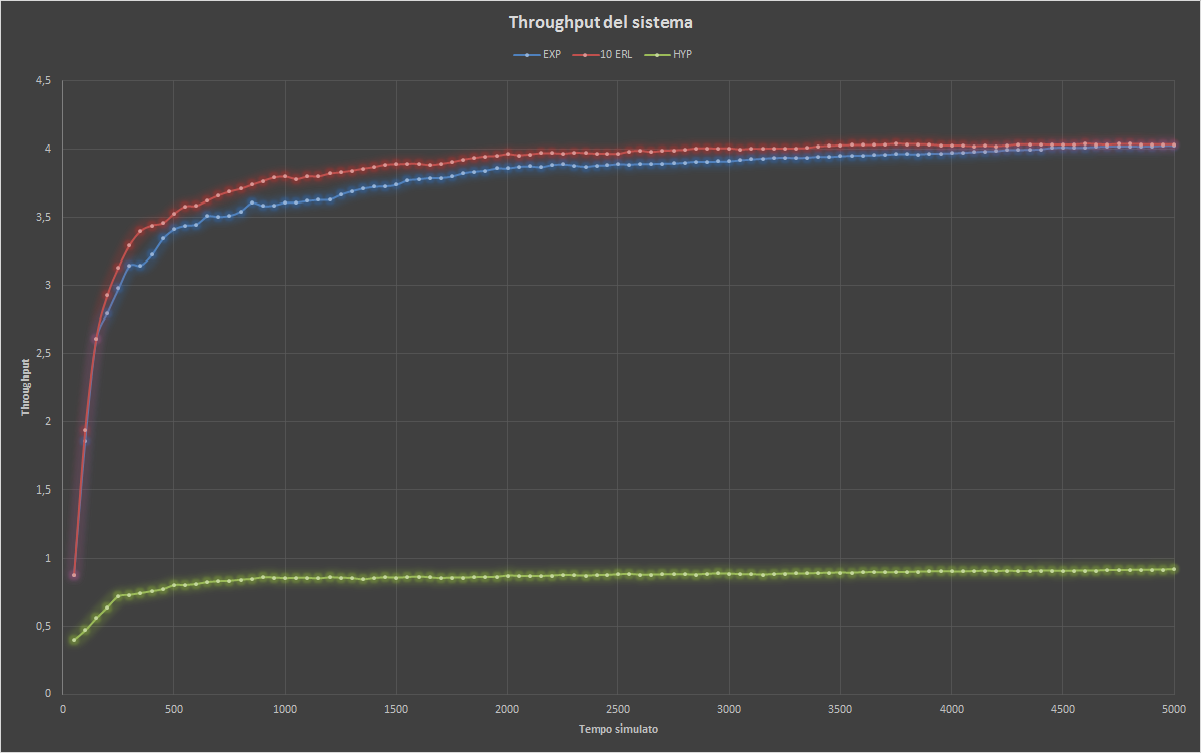
\includegraphics[scale=0.45]{img/throughput.png}
 \caption[Throughput del sistema instabile]{Throughput del sistema instabile}
 \label{fig:Throughput del sistema instabile}
\end{figure}

Anche in questo caso si nota la notevole differenza dello useful throughput  del caso 
iperesponenziale da quelli esponenziali e 10-erlang, i quali coincidono per valori di run  
simulativi molto alti.
Lo useful throughput \'e l'unico indice di prestazione che presenta un andamento stazionario 
all'aumentare del tempo di simulazione. Si pu\`o notare dal grafico, infatti, che tale valore di 
stazionariet\`a \'e all'incirca pari a 4 sessioni completate per unit\`a di tempo.


Di seguito sono stati riportati gli intervalli di confidenza stimati per ogni distribuzione. 
\begin{itemize}
 \item \textit{\textbf{Esponenziale}} : $[ 3,66109876 ; 3,83534225 ]$
 \item \textit{\textbf{10 Erlang}} : $[ 3,75592814 ; 3,92657294 ]$
 \item \textit{\textbf{Iperesponenziale}} : $[ 0,84149673 ; 0,87406350 ]$
\end{itemize}

Infine viene riportato l'istogramma relativo allo useful throughput dato che l'unico
indice con comportamento steady-state:

\begin{figure}[H]
 \centering
 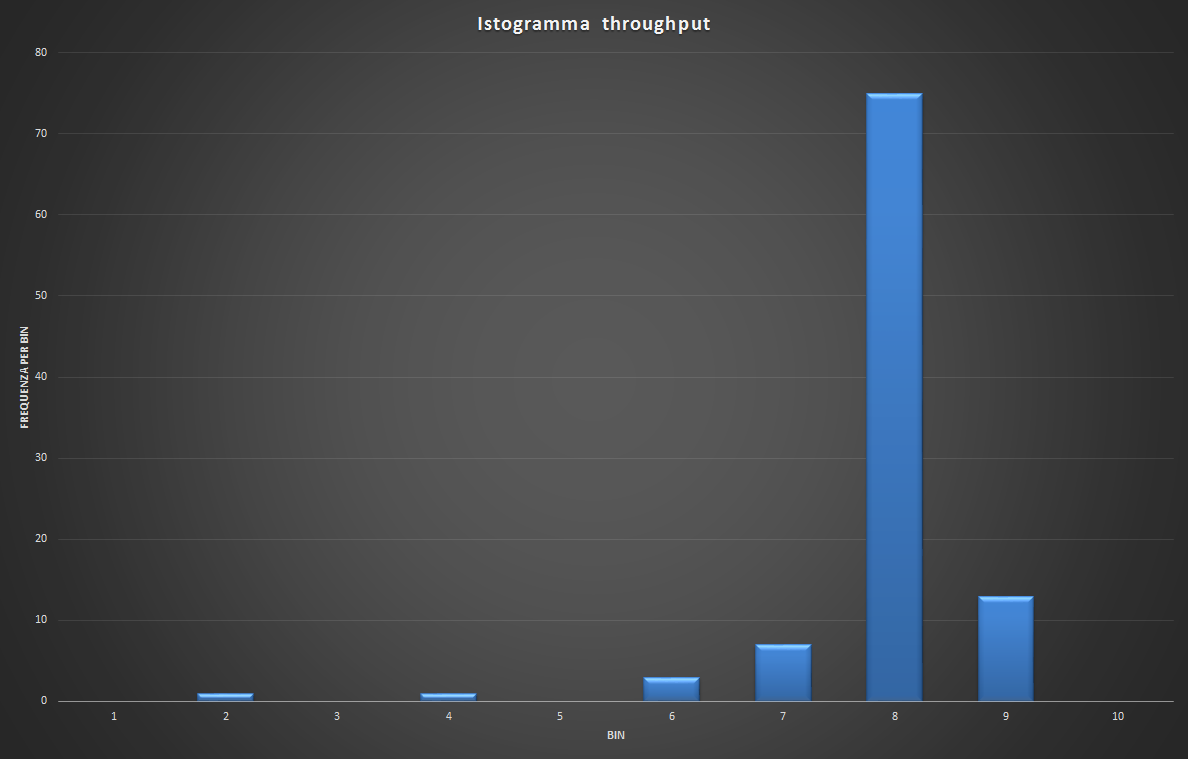
\includegraphics[scale=0.45]{img/istogramma.png}
 \caption[Istogramma del throughtput]{Istogramma del throughtput}
 \label{fig:Istogramma del throughtput}
\end{figure}

\section{Sistema con Overload Management}

Dai risultati illustrati nel caso di sistema senza il meccanismo di \textit{overload 
management} la distribuzione con i tempi di servizio ``peggiore'', ossia con i tempi
di risposta maggiori, \'e risultata quella iperesponenziale. 
Per questa distribuzione, dunque, sono stati effettuati test con la gestione del sovraccarico.
Neanche quando viene applicato l’overload management nel front-end server, gli indici di prestazione
di interesse assumono un comportamento stazionario per run simulativi abbastanza lunghi.
Ci\`o avviene perch\'e anche se in questa situazione il front server ha un'utilizzazione media pi\`u bassa
di 1, e quindi non arriva mai a saturazione, nel momento in cui supera l' 85\% del carico viene impedito l'accesso
a tutte le sessioni, anche quelle gi\`a presenti nel sistema, e di conseguenza la sua coda si svuota, ma
nel momento in cui vengono riabilitati gli arrivi la coda si riempie di nuovo, con l'effetto che tutte le
metriche analizzate avranno oscillazioni non indifferenti rispetto al tempo.

\subsection{Response Time}

Di seguito viene riportato il grafico sul tempo di risposta del sistema con distribuzione dei 
tempi di servizio iperesponenziale del front-end server:

\begin{figure}[H]
 \centering
 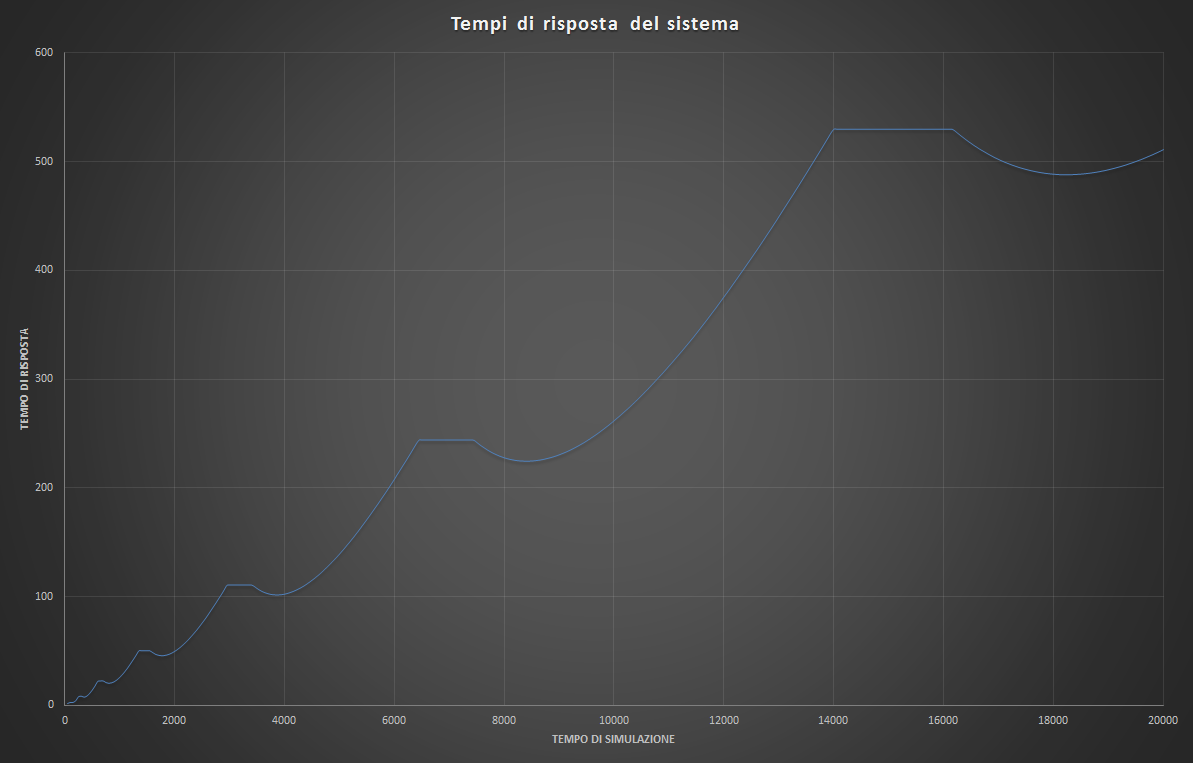
\includegraphics[scale=0.45]{img/responseOM.png}
 \caption[Tempo di risposta del sistema con distribuzione iperesponenziale e overload management attivo]{Tempo di risposta del sistema con distribuzione iperesponenziale e overload management attivo}
 \label{fig:Tempo di risposta del sistema con distribuzione iperesponenziale e overload management attivo}
\end{figure}

Dal grafico riportato sopra si nota ci\`o che era stato detto in precedenza, ovvero il response time
non si stabilizza ma tende a decrescere nei momenti in cui il sistema blocca gli accessi e cresce di 
nuovo quando vengono consentiti nuovamente.

\subsection{Useful Throughtput}
Il grafico successivo illustra l’andamento dello useful throughput del sistema con i 
parametri sopra citati:
\begin{figure}[H]
 \centering
 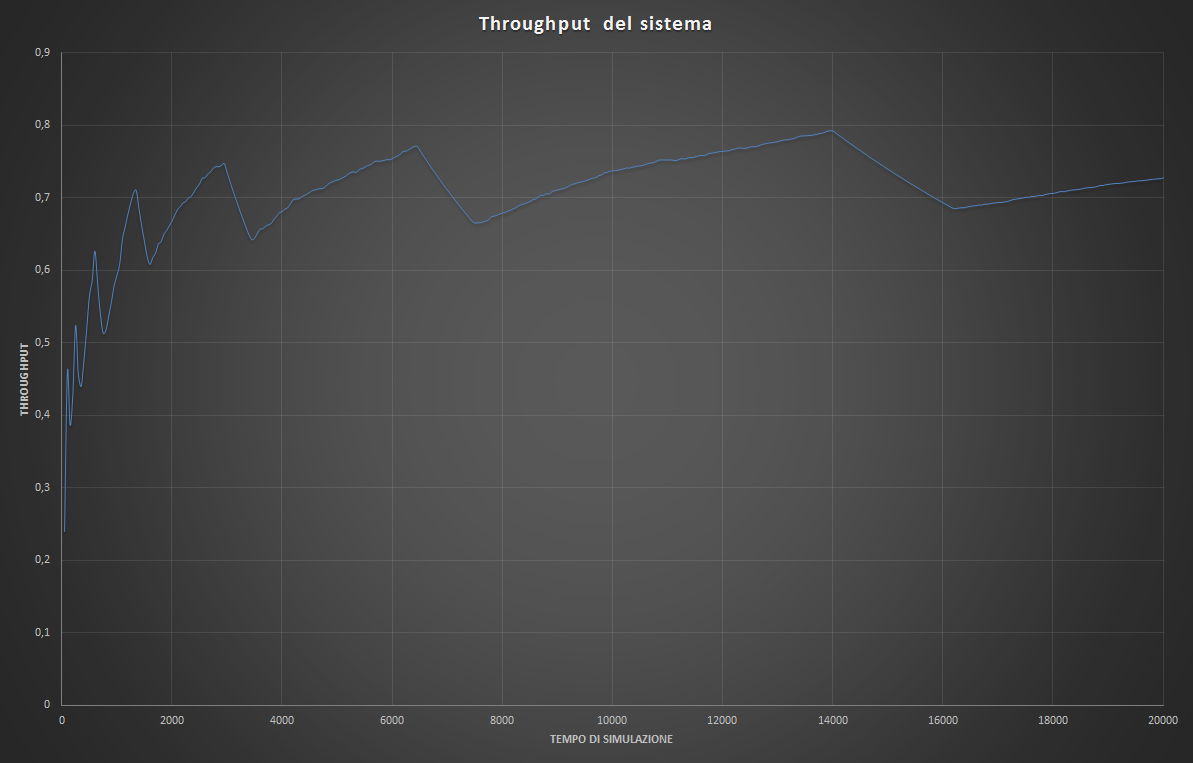
\includegraphics[scale=0.45]{img/throughputOM.png}
 \caption[Throughput del sistema con distribuzione iperesponenziale e overload management attivo]{Throughput del sistema con distribuzione iperesponenziale e overload management attivo}
 \label{fig:Throughput del sistema con distribuzione iperesponenziale e overload management attivo}
\end{figure}
Stessa cosa gi\`a vista per i tempi di risposta avviene nel throughput, anche se in questo caso piano
piano le oscillazioni si vanno ad appiattire.

\subsection{Drop e Aborted Ratio}
Infine vengono riportati gli andamenti degli indici drop ratio e aborted ratio:
\begin{figure}[H]
 \centering
 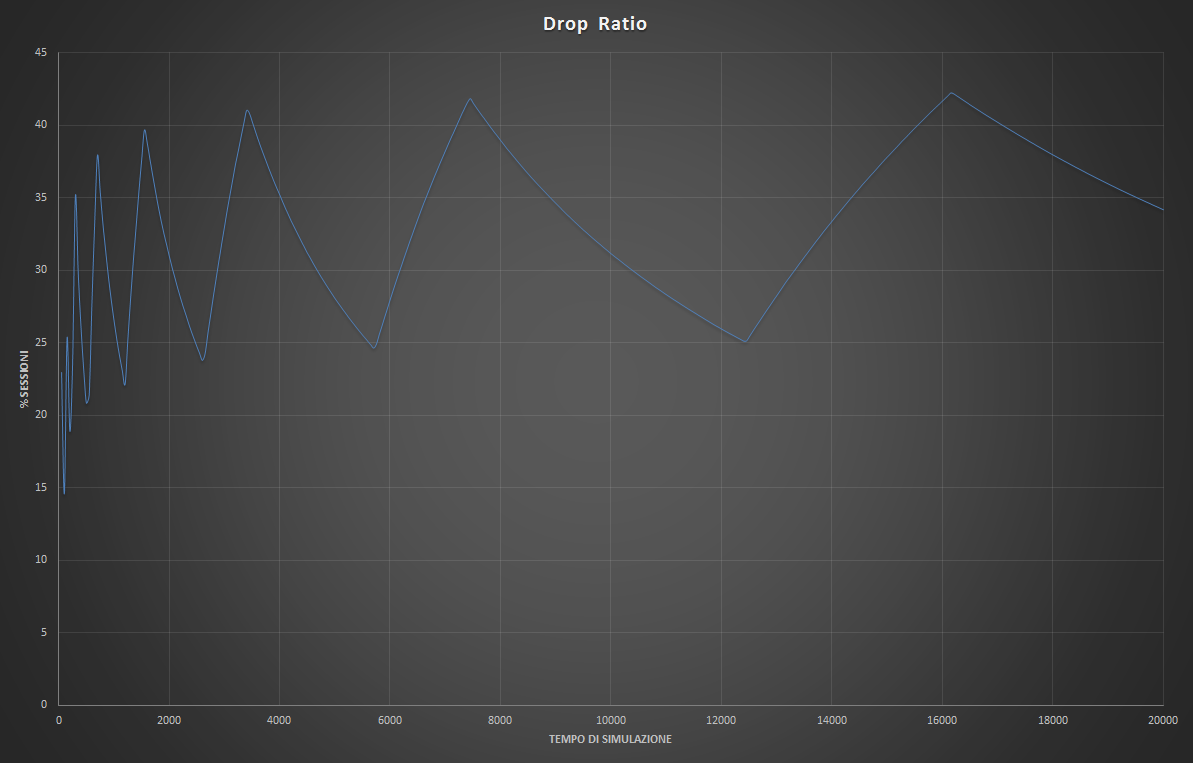
\includegraphics[scale=0.4]{img/dropRatio.png}
 \caption[Drop Ratio]{Drop Ratio}
 \label{fig:Drop Ratio}
\end{figure}
\begin{figure}[H]
 \centering
 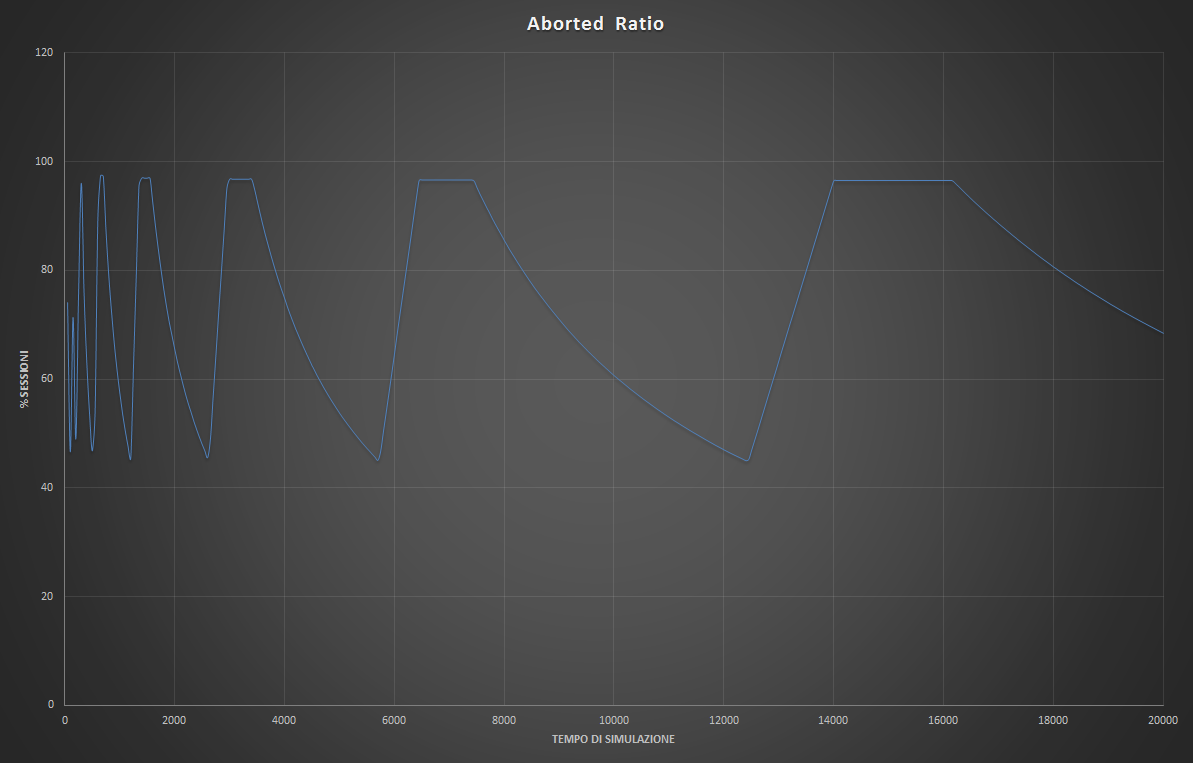
\includegraphics[scale=0.4]{img/abortRatio.png}
 \caption[Aborted Ratio]{Aborted Ratio}
 \label{fig:Aborted Ratio}
\end{figure}
Anche in questi due grafici notiamo come la percentuale di sessioni rifiutate e abortite
oscilli in maniera molto ampia.
\section{Batch means e intervalli di confidenza}

\section{Conclusioni}

In questo progetto \'e stata effettuata l’analisi delle prestazioni di un 
sistema che emula uno scenario di traffico web reale.
Infatti oltre a simulare un comportamento stocastico riguardo sia i tempi di interarrivo delle 
richieste effettuate dai client che ai loro tempi di processamento nei server e di thinking, 
fissati i parametri del sistema dalle specifiche riportate e applicando il meccanismo di 
overload management, il sistema presenta un comportamento simile ai server web reali. 

Si \'e analizzato quindi le prestazioni di tale sistema al variare delle distribuzioni dei tempi di 
servizio, dell applicazione del meccanismo di overload management valutando l’andamento 
degli indici di prestazione di interesse quali lo useful throughput e i tempi di risposta del 
sistema, oltre a valutare il drop ratio e l’abort ratio. A tale scopo è stato utilizzato un 
simulatore next-event il quale integra un meccanismo di avanzamento del tempo simulato 
basato sull’occorrenza degli eventi schedulati in apposite strutture dati.